% !TEX root = tesis.tex

\chapter{Detección de partículas energéticas\\ solares con el SciCRT}
\chaptermark{Detección de partículas}
\label{chap:cuatro}
\section{Desempeño del SciCRT como detector de RC}

Estudios sobre el desempeño del SciCRT como detector de rayos cósmicos se encuentran en \cite{ynagai14,ysasai14}, sin embargo hacen la evaluación durante un periodo de tiempo corto y condiciones operacionales distintas a las actuales. En la presente sección enfocaré mis esfuerzos en determinar el desempeño del detector bajo las condiciones actuales de operación, con vistas a determinar su confiabilidad durante un evento de partículas solares y estimar los errores sistemáticos.

Con el fin de alcanzar este objetivo utilicé un código de simulación que incluye las descripción completa del telescopio, el cual fue desarrollado por mi colega Rocío García. Los detalles de esta simulación se presentan en \cite{garcia20}. Algunos puntos que fueron necesarios adaptar para mi análisis son los siguientes:

\begin{itemize}
  \item Considerar siete tipos de partículas diferentes: neutrones, protones, $\mu^{\pm}$, $e^{\pm}$ y rayos $\gamma$.
  \item Utilizar el modelo PARMA como generador de eventos para las distribuciones de energía y de ángulos cenitales.
  \item Los parámetros de entrada del modelo son los correspondientes a la localidad de Sierra Negra y el periodo de observación de Septiembre de \num{2017}.
  \item Todas los espectros de energía de las partículas usadas en la simulación se definen en un rango de \SI{10}{\mega\electronvolt} a \SI{1}{\tera\electronvolt}.
  \item Los propiedades ópticas de los materiales del detector están deshabilitadas para reducir el tiempo de computo.
  \item Se simulan en total \num{3e7} de eventos, los cuales son lanzados al detector desde una esfera de \SI{5}{\metre} de radio.
\end{itemize}

La figura \ref{fig:sim-setup} muestra la geometría usada en la simulación para inyectar las partículas al detector. El cubo azul representa la posición del detector en la simulación, mientras que las partículas son inyectas desde la esfera.

\begin{figure}
        \centering
        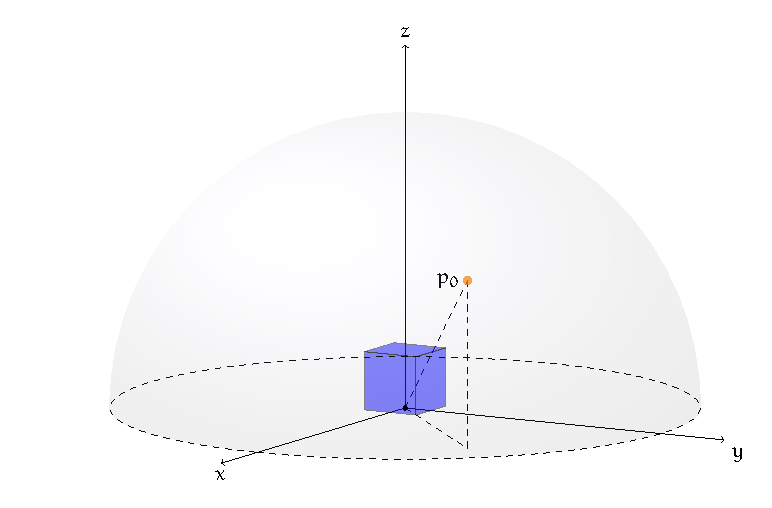
\includegraphics[width=0.75\textwidth]{sim-setup.pdf}
        \caption{Configuración de la simulación en Geant4.}
        \label{fig:sim-setup}
\end{figure}

La condición para que las partículas sean contadas en la simulación es que éstas depositen al menos \SI{7}{\mega\electronvolt} en una barra de cada lado del detector; sin generar señal en las capas dedicadas a la detección de muones. A partir de aquí seleccioné solo los eventos que cumplen con el disparo en el SB \num{3}, que es donde está instalada la electrónica de alta velocidad. El resultado de este análisis se muestra en la figura \ref{fig:total-efficiency}. La línea roja representa la eficiencia de detección de neutrones; mientras que las lineas verde, café, morada, azul y naranja son eficiencias de protones, $\mu^{\pm}$, rayos $\gamma$, positrones y electrones; respectivamente. En todos los casos las eficiencias reportadas son las totales, es decir, están ponderadas con respecto a la distribución angular e incluyen una barra de error. La tasa de eventos total estimada a partir de estas especies es de \SI{3132.31(9480)}{eventos \per\minute}, de los cuales el \SI{84}{\percent} son generados por neutrones.

Las partículas cargadas son rechazadas de manera eficiente usando la señal de anti-coincidencia, sin embargo éstas puede entrar por los lados del detector. Aun así, dado que electrones, positrones y muones depositan en promedio poca energía por barra (aunque tienen una deposición de energía grande en el detector), el umbral de \SI{7}{\mega\electronvolt} constituye una barrera para estas especies. El caso de los protones es más complejo
puesto que pueden tener deposiciones de energía similares a las de los neutrones. De esta forma cerca del \SI{12}{\percent} de los eventos totales son producidos por protones.

De acuerdo con este estudio, el SciCRT tiene una eficiencia de detección grande para rayos $\gamma$ con ángulos mayores a \SI{30}{\degree} y energías superiores a \SI{100}{\mega\electronvolt}; lo cual hace muy limitada su contribución al total de eventos producidos por rayos cósmicos secundarios ya que estos eventos son poco frecuentes.

\begin{figure}
        \centering
        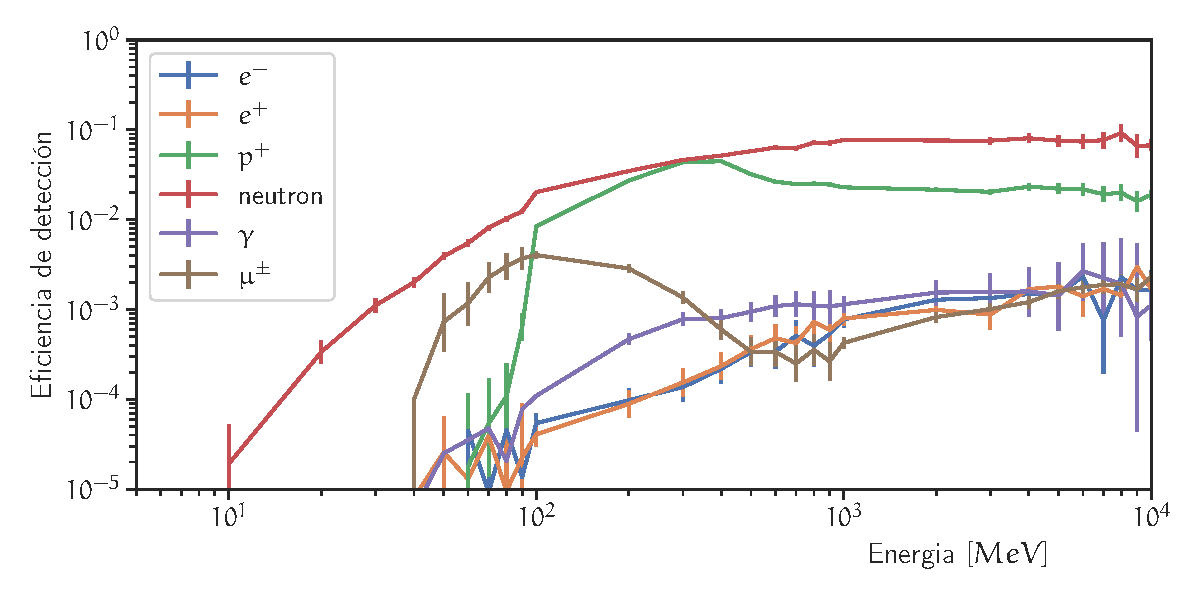
\includegraphics[width=\textwidth]{scibar-efficiency.pdf}
        \caption{Eficiencia de detección del SciCRT para diferentes especies de partículas en función de la energía incidente.}
        \label{fig:total-efficiency}
\end{figure}

El siguiente paso de mi análisis fue comparar la tasa estimada previamente con los datos experimentales. Los datos usados en este parte del análisis provienen del \num{14} de Noviembre de \num{2017}. La tasa de eventos crudos registrada por el telescopio se muestra en la figura \ref{fig:neutron-1pix}. De este modo la tasa media de eventos se estima en: \SI{3841.68(214)}{eventos \per\minute}.

\begin{figure}
        \centering
        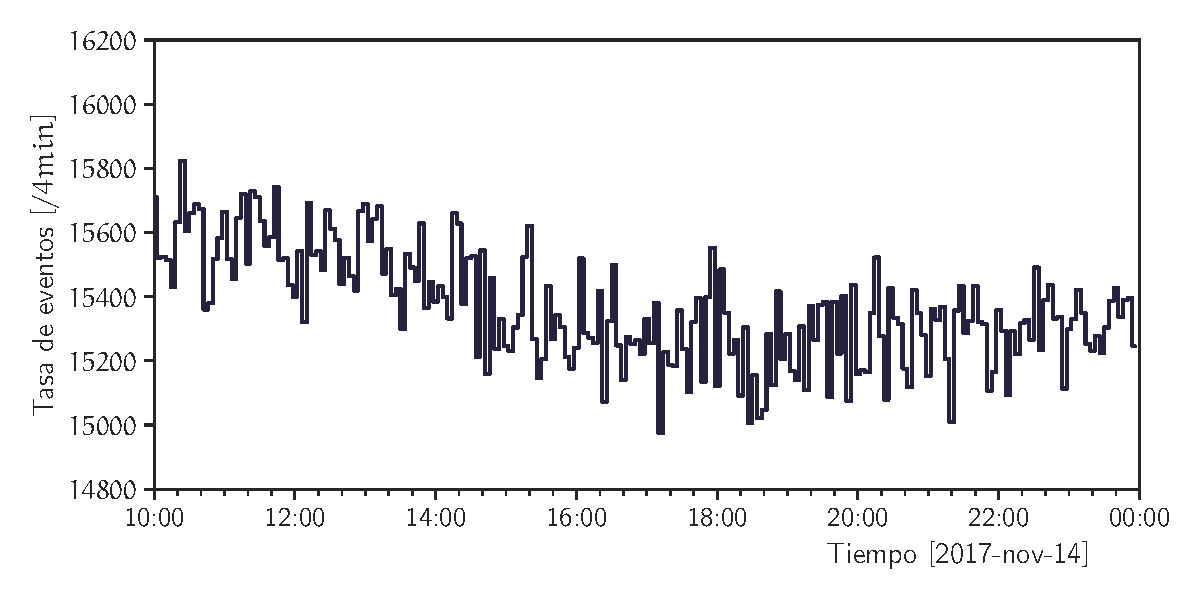
\includegraphics[width=\textwidth]{neutron-171114-1pix.pdf}
        \caption{Tasa de eventos registrada por el SB3 durante el \num{14} de Noviembre de \num{2017}}
        \label{fig:neutron-1pix}
\end{figure}

La diferencia entre la simulación y el experimento es evidente, con un error de \SI{\approx 20}{\percent} tomando como base la simulación. En principio las diferencias deben ser ocasionadas por características del detector no incluidas en la simulación, como pueden ser; las ganancias de los MAPMTs, no linealidades de la electrónica y fluctuaciones debidas a la temperatura, entre otros factores. Dado que las fluctuaciones debidas a la temperatura se deben observar en escalas de tiempo mayores, en primera instancia quedan descartadas como posibles factores que expliquen la discrepancia.

Para poder investigar cualquiera de las posibilidades restantes es necesario reconstruir los eventos registrados por el detector. En resumen este proceso consta de: eliminar el pedestal de las distribuciones de ADC, corregir el efecto de atenuación en las barras y finalmente convertir los valores de ADC en energía depositada.

Una ejemplo de distribución ADC de una de las barras de centelleo se muestra en la figura \ref{fig:neutron-pedestal}. Dos de las características importantes de estas distribuciones son el pico debido a ruido electrónico (pedestal) y el pico de señal (en este caso aproximadamente en \SI{100}{ADC}). Para cada archivo de eventos registrados es necesario estimar el valor del pedestal por barra, ya que éste representa el punto de referencia a partir del cual la electrónica mide la energía depositada. La posición del pedestal de cada barra la calculo a partir de la media de una distribución Gaussiana ajustada al pico principal. La distribución que se muestra en la figura \ref{fig:neutron-pedestal} corresponde a los datos de una barra, acumulados durante una día y a los que se les ha sustraído el pedestal.

\begin{figure}
        \centering
        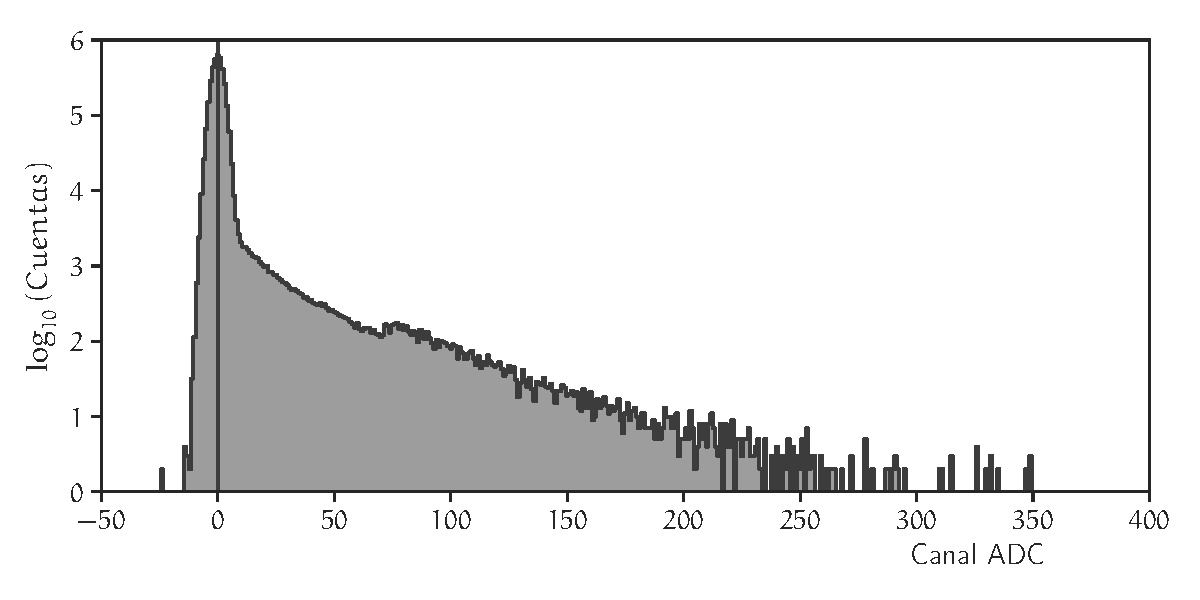
\includegraphics[width=\textwidth]{neutron-ped.pdf}
        \caption{Distribución ADC de una barra de centelleo.}
        \label{fig:neutron-pedestal}
\end{figure}

Posteriormente es necesario corregir los datos de ADC por efectos de la atenuación en la fibra. Este procedimiento se realiza a través de la ecuación \ref{equ:fiber-att}, mencionada previamente. Finalmente los datos de ADC son convertidos a energía depositada usando el mapa de ganancias descrito en \cite{hikimochi16}.

Utilizando los datos de energía depositada, construí distribuciones de energía máxima por traza $E_{max}$, para el periodo de tiempo analizado. El resultado se muestra en la figura \ref{fig:neutron-mindep}, en donde la distribución azul corresponde a las barras del lado Y del SciCRT y la distribución naranja a las del lado X. Estas distribuciones son útiles ya que permiten estudiar el umbral de detección de las barras, y de esta manera nos permiten observar si las diferencias detectadas provienen de la electrónica y/o los MAPMTs. A partir de la figura podemos corroborar que el umbral de detección de las barras es menor a \SI{7}{\mega\electronvolt}, lo cual explica la mayor tasa de eventos en el experimento.

\begin{figure}
        \centering
        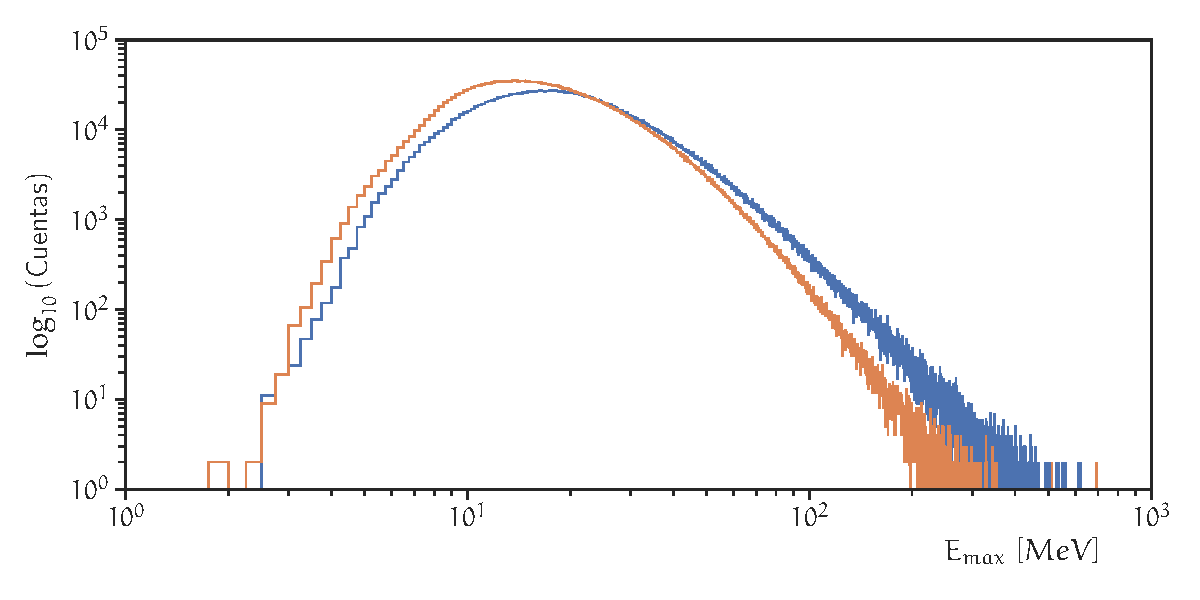
\includegraphics[width=\textwidth]{neutron-mindep.pdf}
        \caption{Distribuciones de energía máxima depositada en una barra de centelleo. La distribución en azul corresponde a las barras del lado Y y la distribución naranja al lado X.}
        \label{fig:neutron-mindep}
\end{figure}

El origen de este fenómeno muy probablemente se debe a unidades de electrónica FE que presentan una ganancia mayor a la del promedio, y por lo tanto permiten registrar eventos de menor energía. La figura \ref{fig:scibar-threshold} permite comprobar este comportamiento. En ella he obtenido las mismas distribuciones de energía máxima depositada, pero en esta ocasión clasificándolas de acuerdo al número de MAPMT donde se detecto el evento. El panel izquierdo muestra en total \num{28} distribuciones, correspondientes a cada uno de los MAPMTs que comprenden el SB3. Se puede apreciar de esta gráfica que la distribución de cada MAPMT inicia en un valor de energía diferente, lo cual apunta a diferencias en el umbral detección. Para observar más claramente este efecto, el panel derecho muestra las distribuciones acumuladas; a partir de las cuales podemos calcular un umbral promedio de \SI{5}{\mega\electronvolt}.

\begin{figure}
        \centering
        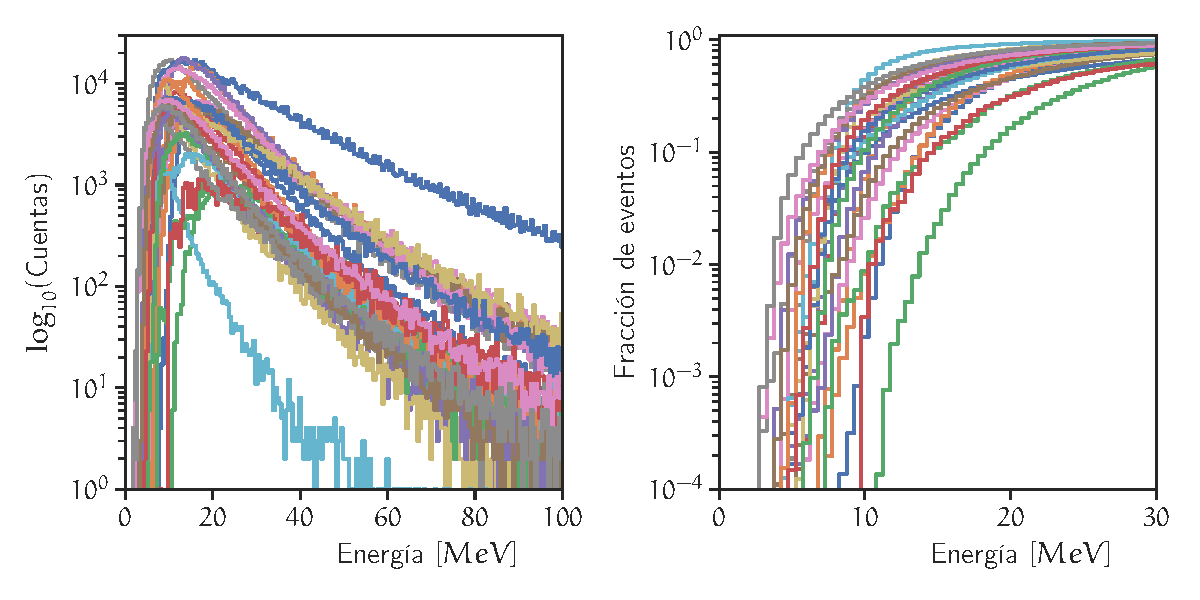
\includegraphics[width=\textwidth]{scibar-threshold.pdf}
        \caption{Distribuciones de energía máxima depositada en una barra de centelleo, clasificadas de acuerdo al MAPMT que registra la señal. El panel izquierdo muestra la distribución de cada fotosensor, mientras que el panel derecho muestra las distribuciones acumuladas.}
        \label{fig:scibar-threshold}
\end{figure}

No obstante, el efecto de este menor umbral solo afecta una pequeña cantidad de eventos; ya que la razón entre el número de eventos que no superan el umbral de \SI{7}{\mega\electronvolt} y los que si solo superan es tan solo del \SI{3.5}{\percent}. Esto podría indicar que el número de canales en la electrónica que permiten el paso de eventos de menor energía es muy pequeño. Luego entonces podemos considerar todos los eventos por debajo de \SI{7}{\mega\electronvolt} como hits accidentales y eliminarlos de nuestro análisis. Finalmente podemos estimar la tasa de eventos del experimento en: \SI{3178.40(177)}{eventos \per\minute}, lo cual concuerda con la simulación dentro de la incertidumbre asociada.

\subsection{Estabilidad del detector}

Para finalizar esta sección presentaré un análisis sobre la operación estable del telescopio. Dado que el SciCRT se encuentra operando en alta montaña, bajo condiciones atmosféricas severas, una parte importante de nuestro trabajo en sitio ha sido el desarrollo e instalación de la infraestructura necesaria. Esto incluye sistemas de respaldo de alimentación eléctrica (banco de baterías y fuente de alimentación ininterrumpida) y sistema de ventilación para favorecer la disipación de calor de la electrónica. La figura \ref{fig:muon-monthly} presenta un ejemplo de la operación estable del detector durante el mes de febrero de \num{2020}. En esta figura se muestran los datos del número de eventos por hora registrados en las capas de muones en color azul oscuro, mientras que la linea azul claro presenta los datos del NM de la Ciudad de México. A fin de presentar ambas gráficas en la misma escala, sume \SI{e6} cuentas a los datos del NM. De la gráfica se puede observar que ambas series de tiempo siguen la misma evolución en el tiempo, lo cual es notable para en el caso de un detector operando a la altura de Sierra Negra ya que los NMs son instrumentos ampliamente usados en el estudio de RC debido a su estabilidad.

\begin{figure}
        \centering
        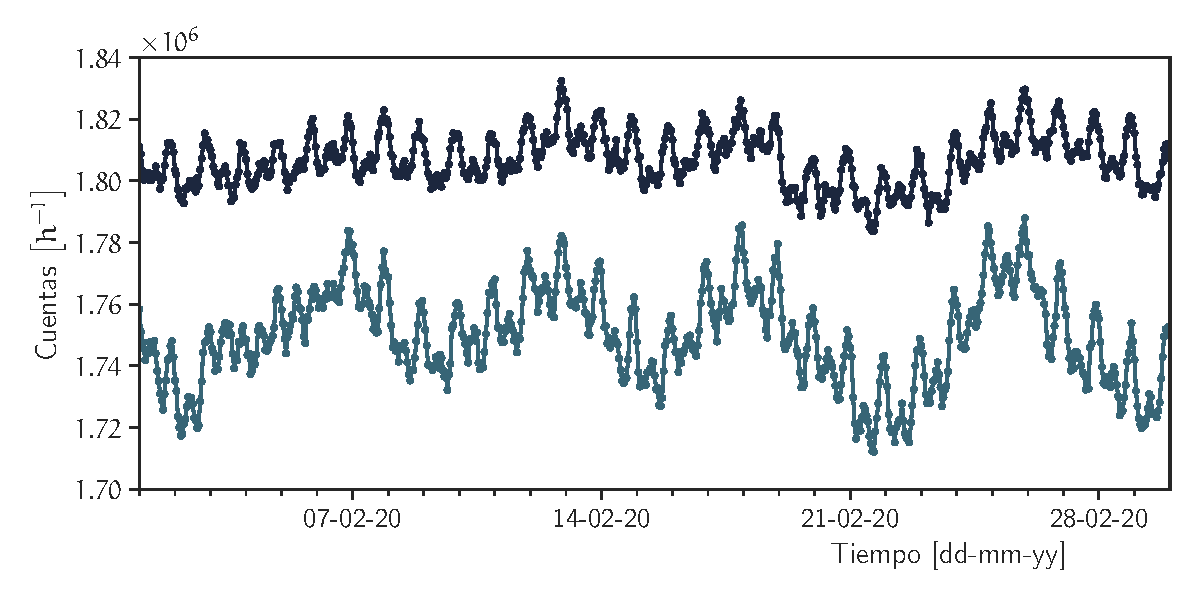
\includegraphics[width=\textwidth]{muon-monthly.pdf}
        \caption{Total de eventos de muones registrados durante Febrero \num{2020} por el SciCRT (linea azul oscura) en comparación con datos del NM de la Ciudad de México (línea azul claro).}
        \label{fig:muon-monthly}
\end{figure}

De forma simular la figura \ref{fig:neutron-monthly} muestra el número de eventos por hora de las capas de neutrones. En este punto es importante aclarar que, debido al gran volumen de datos que registra el SB3, la adquisición en esta capa del detector se detiene por las noches para poder comprimir los archivos registrados. Esto explica las discontinuidades que se observan en la gráfica. A pesar de esta limitante, se pueden notar de la figura que la serie de tiempo sigue la misma tendencia de las otras mencionadas previamente.

\begin{figure}
        \centering
        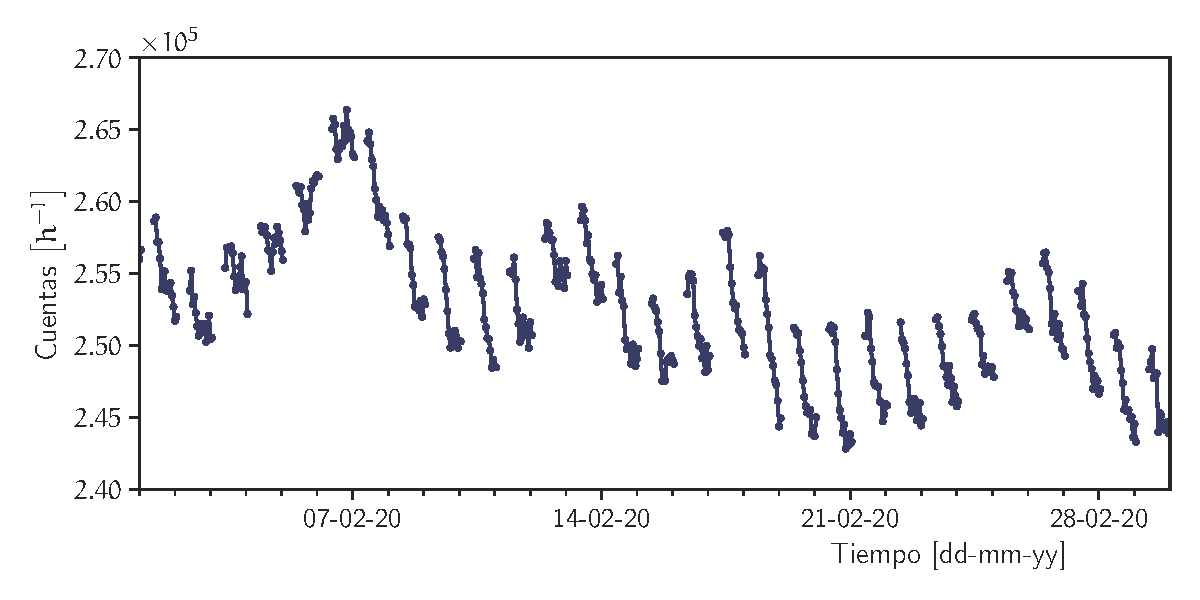
\includegraphics[width=\textwidth]{neutron-monthly.pdf}
        \caption{Total de eventos de partículas neutras registrados durante Febrero \num{2020} por el SciCRT.}
        \label{fig:neutron-monthly}
\end{figure}

Por otra parte, ya que una parte significativa del análisis con los datos de neutrones está relacionada con la deposición de energía en las barras, un estudio de estabilidad requiere monitorear las ganancia de los MAPMTs en función del tiempo. La figura \ref{fig:mip-stability} muestra el resultado de esta análisis para los MAPMTs en las capas de neutrones, durante un periodo de tres; de Diciembre \num{2019} a Febrero \num{2020}. Para calcular la ganancia de los MAPMTs, dado que el pico de señal no es muy prominente, el procedimiento análisis es el siguiente:

\begin{enumerate}
  \item Usando las distribuciones de ADC de cada barra y calcular los pedestales (ver figura \ref{fig:neutron-pedestal}).
  \item Ajustar una función exponencial negativa a la región de \num{15} a \SI{70}{ADC} posterior al pico del pedestal.
  \item Sustraer el pedestal y función exponencial de la distribución de la barra.
  \item Estimar la posición del pico de la señal.
\end{enumerate}

El paso final se puede realizar ajustando una distribución al histograma resultado o calculando la moda del mismo. Por simplicidad del algoritmo utilicé la moda del histograma, sin embargo, resultados similares se pueden obtener ajustando una distribución. La desventaja de usar la moda es que este es parámetro muy sensible a la estadística del histograma, lo cual contrarreste calculando la ganancia en periodos de tres días. El panel superior de la figura \ref{fig:mip-stability} muestra la variación de la ganancia en el tiempo para uno de los MAPMTs del SB3. Como se observa en la figura, la ganancia tiene fluctuaciones considerables durante el periodo, muy probablemente causadas por efectos de temperatura \cite{knitta04}. No obstante, la mayoría de las variaciones están en el intervalo del \SI{\pm 1.0}{\percent} (área sombreada en verde oscuro) y ninguna sobrepasa \SI{\pm 2.0}{\percent} (área sombreada en verde claro).

Finalmente el panel inferior muestra la distribución para todo los MAPMTs en el SB3 durante el periodo de tres meses. De la figura se puede concluir que, a pesar de las condiciones atmosféricas de Sierra Negra, todas las variaciones se encuentran en el rango de \SI{\pm 2.5}{\percent}.

\begin{figure}
        \centering
        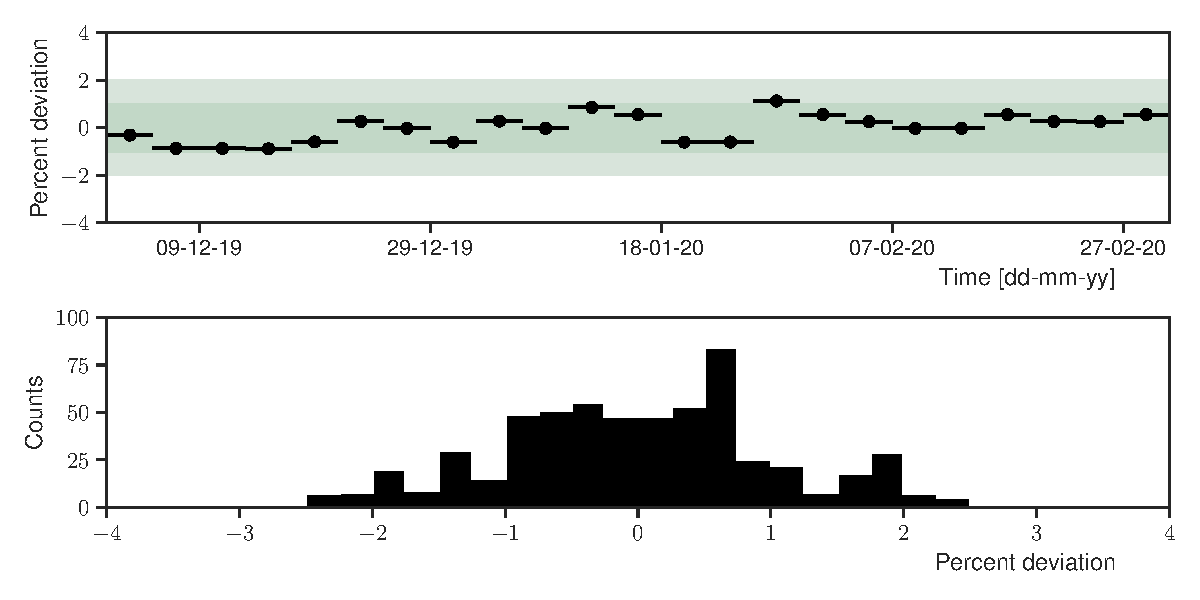
\includegraphics[width=\textwidth]{neutron-mip_stability.pdf}
        \caption{Estabilidad de la ganancia de los MAPMTs durante un periodo de tres meses. El panel superior muestra la variación en el tiempo de uno de los MAPMT. Las áreas sombreadas corresponden con las variaciones de \SI{\pm 1}{\percent} y \SI{\pm 2}{\percent}. El panel inferior es la distribución de todos los MAPMTs.}
        \label{fig:mip-stability}
\end{figure}

\section{Observación de partículas solares}

\begin{figure}
        \centering
        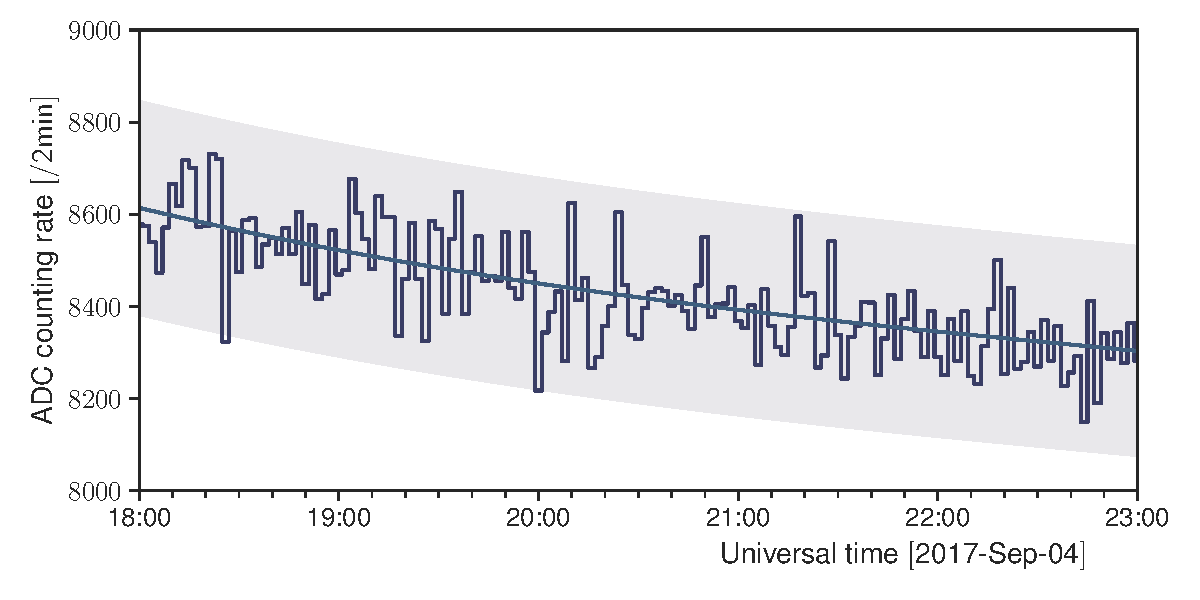
\includegraphics[width=\textwidth]{neutron-170904.pdf}
        \caption{Perfil temporal de eventos registrados por el \emph{SciCRT} el \num{4} de Septiembre de \num{2017}. El área sombreada representa el nivel de $3.0\sigma$.}
        \label{fig:september-04}
\end{figure}

\begin{figure}
        \centering
        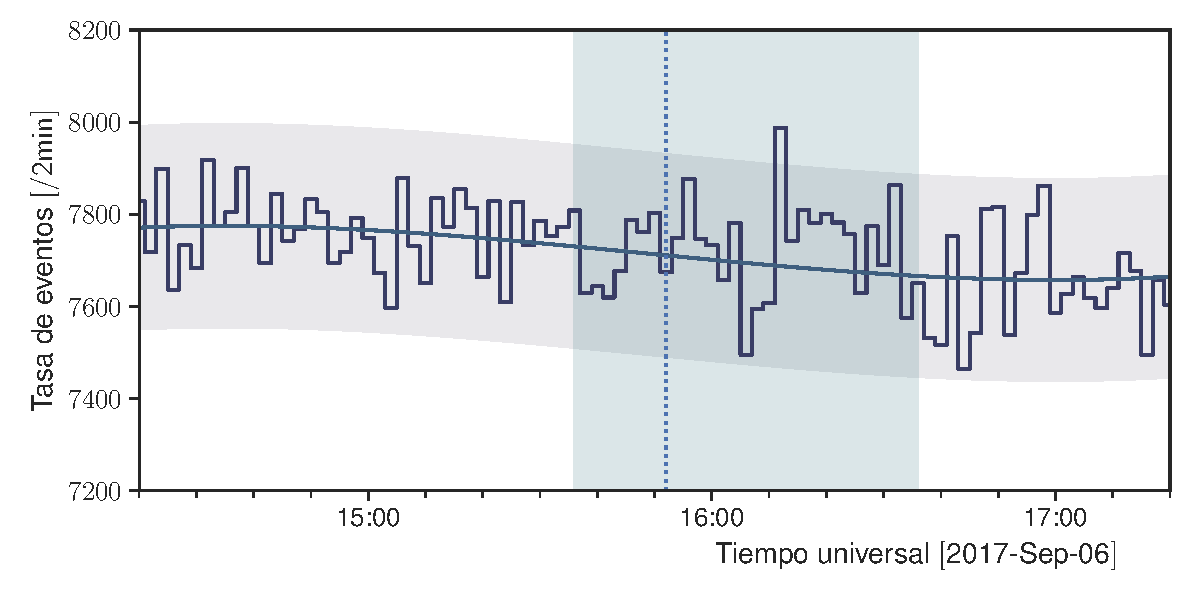
\includegraphics[width=\textwidth]{neutron-170906.pdf}
        \caption{Perfil temporal de eventos registrados por el \emph{SciCRT} el \num{4} de Septiembre de \num{2017}. El área sombreada representa el nivel de $3.0\sigma$..}
        \label{fig:september-06}
\end{figure}
